% -----------------------------------------------------------------------------------
% Document Class and Basic Setup
% -----------------------------------------------------------------------------------
\documentclass[12pt]{extreport}

% -----------------------------------------------------------------------------------
% Packages
% -----------------------------------------------------------------------------------
\usepackage[utf8]{inputenc}
\usepackage[T1]{fontenc}
\usepackage[table,xcdraw]{xcolor}
\usepackage{amsmath, amsfonts, amssymb, amsthm}
\usepackage{graphicx}
\usepackage{float}
\usepackage{geometry}
\usepackage{caption}
\usepackage{subcaption}
\usepackage{booktabs}
\usepackage{array}
\usepackage{url}
\usepackage{hyperref}
\hypersetup{colorlinks=true, linkcolor=blue, citecolor=blue, urlcolor=blue}
\geometry{textwidth=17cm, textheight=23cm}

% -----------------------------------------------------------------------------------
% TikZ
% -----------------------------------------------------------------------------------
\usepackage{tikz}
\usetikzlibrary{positioning}

% -----------------------------------------------------------------------------------
% Theorems and Environments
% -----------------------------------------------------------------------------------
\theoremstyle{definition}
\newtheorem{prob}{Problem}
\renewcommand{\baselinestretch}{1.25}

% -----------------------------------------------------------------------------------
% Document Start
% -----------------------------------------------------------------------------------
\begin{document}

% -----------------------------------------------------------------------------------
% Title Page
% -----------------------------------------------------------------------------------
\begin{figure}[H]
    \centering
    
\includegraphics[height=3cm]{Logo.png} % Replace with your logo image
\end{figure}

\begin{center}
    \textbf{\Large Faculty of Sciences}\\
    \textbf{\large Faculty of Mathematics, Statistics, and Computer Science}\\[0.3cm]
    \textbf{\LARGE Stochastic Processes Mini Project 1}\\
    \vspace{0.2cm}
    \textbf{Due Date: Sunday, 20th AprilM}\\
    \rule{\textwidth}{0.4pt}
\end{center}

\vspace{1cm}

% -----------------------------------------------------------------------------------
% Pierre-Simon Laplace Quote
% -----------------------------------------------------------------------------------
\begin{quote}
    \centering
    \emph{Probability theory is nothing but common sense reduced to calculation.}\\[1ex]
    \textbf{Pierre-Simon Laplace (1749--1827)}
\end{quote}

\vspace{1.0cm}

% -----------------------------------------------------------------------------------
% Problem Statement
% -----------------------------------------------------------------------------------
\section*{Introduction to Decision-Theoretic Planning}

This mini-project introduces the basic idea of Markov Decision Processes (MDPs), which are the foundation of reinforcement learning. Through a simple grid-world environment, we explore how an agent makes decisions to maximize long-term rewards under different terminal state assumptions.

\section*{Markov Reward Process (MRP)}

You encounter the \textit{Markov Chain} in the course as a model for sequences of states with stochastic transitions. A \textit{Markov Reward Process} (MRP) is a generalization of this model that incorporates a reward structure. It allows for evaluating not only how states evolve over time, but also the expected returns associated with those transitions — a key idea in reinforcement learning and decision-theoretic planning.

\bigskip

\begin{center}
\fcolorbox{blue!80!black}{blue!10}{
\parbox{0.95\textwidth}{
\textbf{Definition}\\
A \textbf{Markov Reward Process} is a tuple $\langle \mathcal{S}, \mathcal{P}, \mathcal{R}, \gamma \rangle$, where:
\begin{itemize}
  \item[$\blacktriangleright$] $\mathcal{S}$ is a finite set of states.
  \item[$\blacktriangleright$] $\mathcal{P}$ is the state transition probability matrix:
  \[
  \mathcal{P}_{ss'} = \mathbb{P}[S_{t+1} = s' \mid S_t = s].
  \]
  \item[$\blacktriangleright$] $\mathcal{R}$ is a reward function:
  \[
  \mathcal{R}_s = \mathbb{E}[R_{t+1} \mid S_t = s].
  \]
  \item[$\blacktriangleright$] $\gamma$ is a discount factor, where $\gamma \in [0, 1]$.
\end{itemize}
}
}
\end{center}

\bigskip

\begin{center}
\fcolorbox{blue!80!black}{blue!10}{
\parbox{0.95\textwidth}{
\textbf{Definition}\\
The \textbf{return} $G_t$ is the total discounted reward from time-step $t$:
\[
G_t = R_{t+1} + \gamma R_{t+2} + \gamma^2 R_{t+3} + \dots = \sum_{k=0}^{\infty} \gamma^k R_{t+k+1}
\]

\begin{itemize}
  \item[$\blacktriangleright$] The \textit{discount} $\gamma \in [0, 1]$ is the present value of future rewards.
  \item[$\blacktriangleright$] The value of receiving reward $R$ after $k + 1$ time-steps is $\gamma^k R$.
  \item[$\blacktriangleright$] This formulation values immediate reward over delayed reward:
  \begin{itemize}
    \item $\gamma$ close to $0$ leads to ``myopic'' evaluation.
    \item $\gamma$ close to $1$ leads to ``far-sighted'' evaluation.
  \end{itemize}
\end{itemize}
}
}
\end{center}

\bigskip

\noindent We now define the \textit{state value function} \( v(s) \), which serves as a measure of the long-term value of a given state \( s \) in a Markov Reward Process. Intuitively, it captures the expected return when starting from state \( s \) and following the dynamics of the MRP thereafter.

\begin{center}
\fcolorbox{blue!80!black}{blue!10}{
\parbox{0.8\textwidth}{
The \textbf{state value function} \( v(s) \) of an MRP is the expected return starting from state \( s \):
\[
v(s) = \mathbb{E}[G_t \mid S_t = s]
\]
}
}
\end{center}

\noindent The value function \( v(s) = \mathbb{E}[G_t \mid S_t = s] \) captures the expected return starting from state \( s \). 

\newpage

\bigskip

\noindent\textbf{Task 1.} Derive a recursive expression for the value function \( v(s) \) by breaking down the return \( G_t \) into two parts:
\begin{itemize}
  \item the immediate reward received after being in state \( s \)
  \item the discounted value of the successor state
\end{itemize}

\noindent Use the definition of return, the Markov property, and properties of expectation to express \( v(s) \) in terms of itself.

\medskip

\noindent This leads to a recursive formulation known as the \textit{Bellman Equation for MRP}.

\bigskip

\noindent\textbf{Task 2.} Express the recursive formulation from Task 1 in matrix form.

\begin{itemize}
  \item Define a vector containing the value of each state.
  \item Represent transitions between states using a matrix.
  \item Write the equation that relates these components linearly.
\end{itemize}

\noindent Solve the resulting linear system to compute the value function for all states.

\noindent In other words, solving the Bellman equation in matrix form yields an explicit expression for the state value vector \( \mathbf{v} \) in terms of the reward vector and the transition dynamics of the process.

\section*{Markov Decision Process (MDP)}

A \textit{Markov Decision Process} (MDP) extends a Markov Reward Process by introducing \textit{actions}. In an MDP, the agent makes decisions that influence both the next state and the received reward. It provides a mathematical framework for modeling sequential decision-making in stochastic environments where all states satisfy the Markov property.

\bigskip

\begin{center}
\fcolorbox{blue!80!black}{blue!10}{
\parbox{0.95\textwidth}{
\textbf{Definition}\\
A \textbf{Markov Decision Process} is a tuple $\langle \mathcal{S}, \mathcal{A}, \mathcal{P}, \mathcal{R}, \gamma \rangle$, where:
\begin{itemize}
  \item[$\blacktriangleright$] \( \mathcal{S} \) is a finite set of states.
  \item[$\blacktriangleright$] \( \mathcal{A} \) is a finite set of actions.
  \item[$\blacktriangleright$] \( \mathcal{P} \) is a state transition probability function:
  \[
  \mathcal{P}^a_{ss'} = \mathbb{P}[S_{t+1} = s' \mid S_t = s, A_t = a].
  \]
  \item[$\blacktriangleright$] \( \mathcal{R} \) is a reward function:
  \[
  \mathcal{R}^a_s = \mathbb{E}[R_{t+1} \mid S_t = s, A_t = a].
  \]
  \item[$\blacktriangleright$] \( \gamma \in [0,1] \) is a discount factor.
\end{itemize}
}
}
\end{center}

\bigskip

\noindent\textbf{Important Note.} In a grid-based environment, each action (e.g., \textit{up}, \textit{down}, \textit{left}, \textit{right}) defines its own transition probability distribution over the next states. That is, the probability of reaching a specific successor state depends not only on the current state but also on the action taken.

\medskip

This means that for each action \( a \in \mathcal{A} \), there is a separate transition matrix \( \mathbf{P}^a \in \mathbb{R}^{|\mathcal{S}| \times |\mathcal{S}|} \), where the entry \( \mathbf{P}^a_{ss'} \) represents the probability of transitioning from state \( s \) to state \( s' \) when action \( a \) is taken.

\medskip

In contrast to Markov Reward Processes (MRPs), where the transition dynamics are governed by a single matrix \( \mathbf{P} \), MDPs maintain one transition matrix per action. This structure is essential for defining how an agent's behavior (via a policy) influences state evolution and expected rewards.

\bigskip

\noindent\textbf{Policy:} In a MDP, a \textit{policy} defines the agent's behavior by specifying how actions are selected in each state. A policy maps each state to a probability distribution over actions, describing the likelihood of taking each action in that state.

\begin{center}
\fcolorbox{blue!80!black}{blue!10}{
\parbox{0.8\textwidth}{
\textbf{Definition}\\
A \textbf{policy} \( \pi \) is a distribution over actions given states:
\[
\pi(a \mid s) = \mathbb{P}[A_t = a \mid S_t = s]
\]
}
}
\end{center}

\noindent Important properties of policies:
\begin{itemize}
  \item A policy fully defines the behavior of an agent.
  \item In MDPs, policies depend only on the current state — not on the full history.
  \item Policies can be:
    \begin{itemize}
      \item \textit{Deterministic}, selecting one specific action per state.
      \item \textit{Stochastic}, assigning a probability distribution over possible actions.
    \end{itemize}
\end{itemize}

\bigskip

\noindent Once a policy \( \pi \) is fixed, the MDP behaves like a Markov Reward Process (MRP). That is:

\begin{itemize}
  \item Given an MDP \( \mathcal{M} = \langle \mathcal{S}, \mathcal{A}, \mathcal{P}, \mathcal{R}, \gamma \rangle \) and a policy \( \pi \),
  \item The resulting state sequence \( S_1, S_2, \ldots \) forms a Markov process defined by \( \langle \mathcal{S}, \mathcal{P}^\pi \rangle \),
  \item And the state–reward sequence \( S_1, R_1, S_2, R_2, \ldots \) forms a Markov Reward Process: 
  \[
  \langle \mathcal{S}, \mathcal{P}^\pi, \mathcal{R}^\pi, \gamma \rangle
  \]
\end{itemize}

\noindent where:
\[
\mathcal{P}^\pi_{ss'} = \sum_{a \in \mathcal{A}} \pi(a \mid s) \, \mathcal{P}^a_{ss'}
\quad \text{and} \quad
\mathcal{R}^\pi_s = \sum_{a \in \mathcal{A}} \pi(a \mid s) \, \mathcal{R}^a_s
\]

\noindent These define the transition and reward dynamics under policy \( \pi \), allowing the MDP to be evaluated as an MRP — a critical step in policy evaluation and value function analysis.

\bigskip

\noindent Once an agent follows a fixed policy \( \pi \), we can evaluate how good each state is under that policy. This is captured by the \textit{state-value function}.

\begin{center}
\fcolorbox{blue!80!black}{blue!10}{
\parbox{0.85\textwidth}{
\textbf{Definition}\\
The \textbf{state-value function} \( v_\pi(s) \) of an MDP is the expected return starting from state \( s \), and then following policy \( \pi \):
\[
v_\pi(s) = \mathbb{E}_\pi \left[ G_t \mid S_t = s \right]
\]

\medskip

The \textbf{action-value function} \( q_\pi(s, a) \) is the expected return starting from state \( s \), taking action \( a \), and then following policy \( \pi \):
\[
q_\pi(s, a) = \mathbb{E}_\pi \left[ G_t \mid S_t = s, A_t = a \right]
\]
}
}
\end{center}

\bigskip


\noindent There exists a fundamental relationship between the state-value function \( v_\pi(s) \) and the action-value function \( q_\pi(s, a) \), expressed by the following two equations:

\[
v_\pi(s) = \sum_{a \in \mathcal{A}} \pi(a \mid s) \, q_\pi(s, a)
\]

\[
q_\pi(s, a) = \mathcal{R}_s^a + \gamma \sum_{s' \in \mathcal{S}} \mathcal{P}^a_{ss'} \, v_\pi(s')
\]

\noindent Substituting the second equation into the first yields the \textit{Bellman Expectation Equation} for \( v_\pi(s) \), which recursively expresses the value function as:

\[
v_\pi(s) = \sum_{a \in \mathcal{A}} \pi(a \mid s) \left( \mathcal{R}_s^a + \gamma \sum_{s' \in \mathcal{S}} \mathcal{P}^a_{ss'} \, v_\pi(s') \right)
\]

\noindent This equation plays a central role in the evaluation of policies and forms the basis of many reinforcement learning algorithms.

\medskip

\noindent For a detailed explanation of why this decomposition holds, see  
\href{https://www.deeplearningwizard.com/deep_learning/deep_reinforcement_learning_pytorch/bellman_mdp/#bellman-expectation-equations}{here}.


\bigskip

\noindent Ultimately, our goal in solving a Markov Decision Process is to find the \textit{optimal state-value function} \( v_*(s) \), which gives the maximum expected return achievable from each state under any policy.

\begin{center}
\fcolorbox{blue!80!black}{blue!10}{
\parbox{0.85\textwidth}{
\textbf{Definition}\\
The \textbf{optimal state-value function} \( v_*(s) \) is the maximum value function over all policies:
\[
v_*(s) = \max_{\pi} v_\pi(s)
\]

\medskip

The \textbf{optimal action-value function} \( q_*(s, a) \) is the maximum action-value function over all policies:
\[
q_*(s, a) = \max_{\pi} q_\pi(s, a)
\]
}
}
\end{center}


\noindent Once the optimal state-value function \( v_*(s) \) or the optimal action-value function \( q_*(s, a) \) is known, it can be used to extract an optimal policy

\bigskip

\noindent Solving for the optimal value function \( v_*(s) \) analytically is generally intractable, especially in environments with large state spaces. Instead, we use iterative methods to approximate \( v_*(s) \). One of the most fundamental algorithms for this purpose is \textit{Value Iteration}.

\medskip

\noindent\textbf{Task 3.} Investigate how the \textbf{Value Iteration} algorithm works to compute the optimal state-value function \( v_*(s) \).  
Formally describe how it iteratively updates estimates of \( v(s) \) based on the Bellman optimality principle, and explain its convergence properties.

\bigskip



\section*{Practical Part: Grid World Environment}

Now that we have studied the theoretical foundations of Markov Decision Processes, our goal is to implement these ideas in a simplified environment.

In this part, we work with a \textit{Grid World}, where each cell corresponds to a unique state. Some of these states provide fixed rewards (positive or negative), while others represent impassable \textit{walls}. The agent can move in four directions: up, down, left, or right — unless blocked by a wall or the edge of the grid.

Below is the grid-world environment we will use throughout this practical section:

\begin{center}
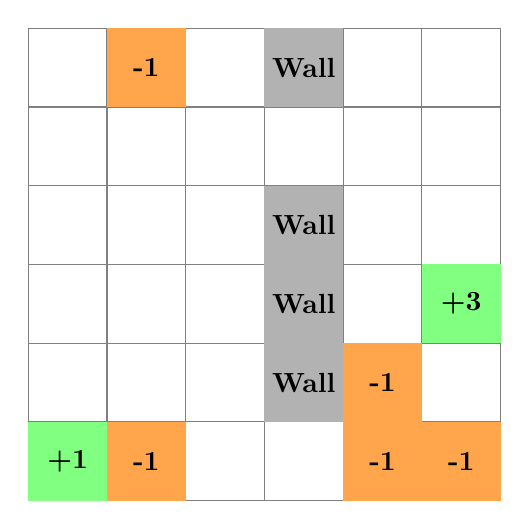
\begin{tikzpicture}
  \def\cellsize{1}
  \foreach \x in {0,...,5} {
    \foreach \y in {0,...,5} {
      \draw[gray] (\x*\cellsize, \y*\cellsize) rectangle ++(\cellsize, \cellsize);
    }
  }

  % Walls
  \foreach \x/\y in {3/1, 3/2, 3/3, 3/5} {
    \fill[gray!60] (\x, \y) rectangle ++(1,1);
    \node at (\x+0.5,\y+0.5) {\textbf{Wall}};
  }

  % +3 Reward
  \fill[green!50] (5, 2) rectangle ++(1,1);
  \node at (5.5, 2.5) {\textbf{+3}};

  % +1 Reward
  \fill[green!50] (0, 0) rectangle ++(1,1);
  \node at (0.5, 0.5) {\textbf{+1}};

  % -1 Rewards
  \foreach \x/\y in {1/0, 4/0, 5/0, 4/1, 1/5} {
    \fill[orange!70] (\x,\y) rectangle ++(1,1);
    \node at (\x+0.5,\y+0.5) {\textbf{-1}};
  }

\end{tikzpicture}
\end{center}

\medskip

\noindent The environment is defined over a $6 \times 6$ grid, where each cell corresponds to a state:

\begin{itemize}
  \item \textbf{White cells} represent normal states with a default reward of $-0.04$ per step.
  \item \textbf{Green cell} provides an immediate reward of $+3$ or $+1$ upon entry.
  \item \textbf{Orange cells} are states with an immediate reward of $-1$ upon entry.
  \item \textbf{Gray cells} are walls and cannot be entered; if the agent attempts to move into a wall, it remains in the same state.
\end{itemize}

\noindent The agent can take one of four actions in each state: \texttt{up}, \texttt{down}, \texttt{left}, or \texttt{right}. The environment follows a \textbf{uniform stochastic transition model}: at each time step, the agent transitions uniformly at random to one of the neighboring directions, regardless of the intended action. That is, each of the four directions is executed with probability \( \frac{1}{4} \). If a selected transition would lead to an invalid state (e.g., into a wall or outside the grid), the agent remains in its current state with no movement and receives \textbf{-0.04 reward} for that step.




\newpage
\noindent\textbf{Task 4.} Implement the Grid World environment by defining the following components:
\begin{itemize}
  \item The state space \( \mathcal{S} \subset \mathbb{Z}^2 \)
  \item The action space \( \mathcal{A} = \{ \texttt{up}, \texttt{down}, \texttt{left}, \texttt{right} \} \)
  \item The reward function \( \mathcal{R}(s) \), including special cases for green and orange cells
  \item The discount factor \( \gamma \in [0,1] \)
  \item The transition probability function \( \mathcal{P}^a_{ss'} = \mathbb{P}[S_{t+1} = s' \mid S_t = s, A_t = a] \) for each action
\end{itemize}

\medskip

\noindent\textbf{Task 5.} Using the \textbf{Value Iteration} algorithm, compute the optimal state-value function \( v_*(s) \) for all states in the grid. Iterate until the value function converges within a small tolerance (e.g., $10^{-4}$).

\medskip

\noindent\textbf{Task 6 (Bonus).} Using the \textbf{action-value function} concept introduced earlier, derive the \textbf{optimal policy} \( \pi_*(s) \). For each state, determine the action that maximizes the expected return by evaluating:
\[
\pi_*(s) = \arg\max_{a \in \mathcal{A}} q_*(s,a)
\]
where \( q_*(s,a) \) is computed using the optimal value function \( v_*(s) \).

\bigskip

\noindent\textbf{Implementation Notes.}

\bigskip

\noindent A code template in the form of a Jupyter notebook is available on the eLearn platform. You may use this template to structure your implementation, but its use is not mandatory. It includes function headers and structural guidance aligned with the tasks defined in this project.

\medskip

\noindent You should submit your code and any additional required files by uploading a single compressed \texttt{.zip} file via eLearn. The file name must follow the format:
\[
\texttt{MiniProject1\_SP\_lastname\_studentid.zip}
\]







\end{document}
